\bookchapter{Rust Basics}\label{ch:rust2}

\section*{Explanation}
This chapter gets you from nothing to small Rust programs that calculate with numbers, use loops and functions, and print results. Everything is explained by comparison with Python, because that is what you know. All programs in this chapter were compiled and run with Rust 1.97 (edition 2024) on the computer that was used to write the book; the output shown is the real output.

\section*{Installing Rust and the first project}
Rust is installed with \textbf{rustup}, the tool that manages compiler versions and extra targets (Chapter~\ref{ch:rust10}). On Ubuntu follow the instructions on \texttt{rust-lang.org}, or install the \verb!rustup! package from the Ubuntu archive; then:
\begin{verbatim}
$ rustup default stable
$ rustc --version
rustc 1.97.0 (2d8144b78 2026-07-07)
$ cargo new hello
    Creating binary (application) `hello` package
$ cd hello
$ cargo run
   Compiling hello v0.1.0 (/home/student/hello)
    Finished `dev` profile [unoptimized + debuginfo] target(s) in 0.18s
     Running `target/debug/hello`
Hello, world!
\end{verbatim}
\textbf{Cargo} is the build tool and package manager of Rust, it does the work of \verb!pip!, \verb!venv! and a Makefile together. A project (called a \textbf{crate}) has this layout:
\begin{center}
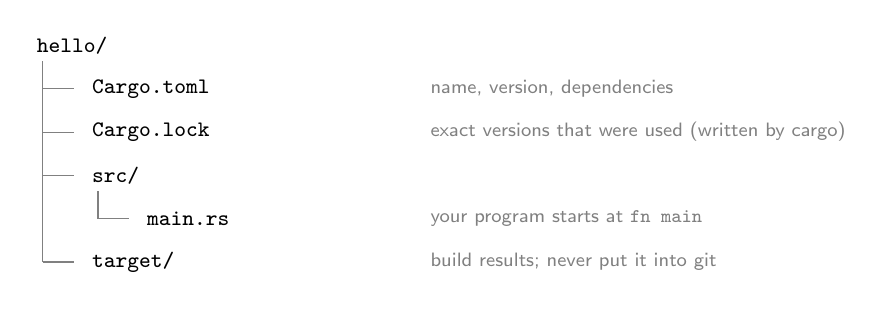
\begin{tikzpicture}[font=\ttfamily\footnotesize,x=1cm,y=1cm]
 \node[anchor=west] at (0,0) {hello/};
 \node[anchor=west] at (0.7,-0.55) {Cargo.toml};  \node[anchor=west,font=\sffamily\scriptsize,gray] at (5,-0.55) {name, version, dependencies};
 \node[anchor=west] at (0.7,-1.1) {Cargo.lock};   \node[anchor=west,font=\sffamily\scriptsize,gray] at (5,-1.1) {exact versions that were used (written by cargo)};
 \node[anchor=west] at (0.7,-1.65) {src/};
 \node[anchor=west] at (1.4,-2.2) {main.rs};      \node[anchor=west,font=\sffamily\scriptsize,gray] at (5,-2.2) {your program starts at \texttt{fn main}};
 \node[anchor=west] at (0.7,-2.75) {target/};     \node[anchor=west,font=\sffamily\scriptsize,gray] at (5,-2.75) {build results; never put it into git};
 \draw[gray] (0.2,-0.2)--(0.2,-2.75) (0.2,-0.55)--(0.6,-0.55) (0.2,-1.1)--(0.6,-1.1) (0.2,-1.65)--(0.6,-1.65) (0.2,-2.75)--(0.6,-2.75) (0.9,-1.85)--(0.9,-2.2)--(1.3,-2.2);
\end{tikzpicture}
\captionof{figure}{The layout that \texttt{cargo new} creates.}
\end{center}
The commands you will use every day:
\begin{center}
\renewcommand{\arraystretch}{1.2}
\begin{tabular}{ll}
\verb!cargo run! & compile (if needed) and run\\
\verb!cargo build --release! & optimised build, in \verb!target/release/!\\
\verb!cargo check! & only check the code, very fast, no program\\
\verb!cargo test! & run the tests (Chapter~\ref{ch:rust5})\\
\verb!cargo fmt! & format the code in the standard style\\
\verb!cargo clippy! & a ``linter'' with advice for better code\\
\verb!cargo add name! & add a dependency to \verb!Cargo.toml!\\
\end{tabular}
\end{center}
The first program, without cargo:
%rs:hello
\begin{verbatim}
fn main() {
    println!("Hello, robot");
}
\end{verbatim}
\verb!fn! defines a function, and the function \verb!main! is where every program starts. The braces \verb!{ }! replace the indentation of Python (indentation is only style in Rust, \verb!cargo fmt! sets it for you). Every statement ends with a semicolon. \verb|println!| is a \textbf{macro} (the exclamation mark tells you): it can take a variable number of arguments and checks the format string at compile time.

\section*{Variables: immutable by default}
%rsmain:vars
\begin{verbatim}
    let speed = 0.5;            // type f64 is inferred
    let name = "K1";            // a string slice
    let mut count = 0;          // mut: may be changed
    count += 1;
    let speed = speed * 2.0;    // shadowing: a NEW variable
    let n: u8 = 200;            // type written out
    println!("{name} {speed} {count} {n}");
\end{verbatim}
This prints \verb!K1 1 1 200!. Three differences to Python: (1) a variable that is not declared \verb!mut! cannot be changed, which prevents a whole class of mistakes (``who changed this value?''); (2) \textbf{shadowing} with a new \verb!let! creates a new variable with the same name, possibly with a new type; (3) every variable has one fixed \textbf{type}, which the compiler infers or you write after a colon. Trying to change an immutable variable is a compile error:
%rsfail:immut
\begin{verbatim}
fn main() {
    let x = 5;
    x = 6;
    println!("{x}");
}
\end{verbatim}
The compiler says \verb!error[E0384]: cannot assign twice to immutable variable `x`!, points at both lines and suggests ``consider making this binding mutable, with \verb!let mut x = 5;!. Constants are written \verb!const MAX_SPEED: f64 = 1.2;! (type required, upper-case name, value known at compile time).

\section*{Numbers and types}
\begin{center}
\renewcommand{\arraystretch}{1.2}
\begin{tabular}{lll}
\textbf{type} & \textbf{meaning} & \textbf{range / precision}\\ \hline
\verb!i8 i16 i32 i64! & signed integers & e.g.\ \verb!i32!: $-2^{31}\dots2^{31}-1$ ($\pm2.1\cdot10^9$)\\
\verb!u8 u16 u32 u64! & unsigned integers & e.g.\ \verb!u8!: $0\dots255$\\
\verb!usize! & unsigned, size of a pointer & indices of arrays and lengths\\
\verb!f32! & floating point, 32 bit & about 7 digits\\
\verb!f64! & floating point, 64 bit & about 15--16 digits (the default)\\
\verb!bool! & \verb!true! or \verb!false! & \\
\verb!char! & one Unicode character & written \verb!'a'!\\
\end{tabular}
\end{center}
Python has one integer type that grows as needed and one \verb!float! (which is an \verb!f64!). Rust integers have a \emph{fixed size}, which is important when a number comes from a sensor or a network packet: a motor ID is a \verb!u8!, a timestamp in microseconds a \verb!u64!, an encoder count an \verb!i32!. There is no automatic conversion between types: \verb!1 + 2.5! is an error, you write \verb!1.0 + 2.5! or convert with \verb!as!.
%rsmain:numbers
\begin{verbatim}
    println!("{}", 7 / 2);            // integers: integer division
    println!("{}", 7.0 / 2.0);        // floats
    println!("{}", -7 % 3);           // remainder keeps the sign
    println!("{}", (-7_i32).rem_euclid(3));  // always 0..2
    println!("{}", 3.99_f64 as i32);  // cuts the decimals
    println!("{}", -1_i32 as u8);     // wraps around
    println!("{}", 300_i32 as u8);    // wraps around
    println!("{}", 255_u8.wrapping_add(1));
    println!("{:?}", 255_u8.checked_add(1));
    println!("{}", 255_u8.saturating_add(1));
    println!("{}", (2.0_f64).sqrt());
    println!("{}", f64::NAN == f64::NAN);
\end{verbatim}
prints, one per line: \verb!3!, \verb!3.5!, \verb!-1!, \verb!2!, \verb!3!, \verb!255!, \verb!44!, \verb!0!, \verb!None!, \verb!255!, \verb!1.4142135623730951!, \verb!false!. Look at the three ways to add to a \verb!u8! that is already $255$:
\begin{center}
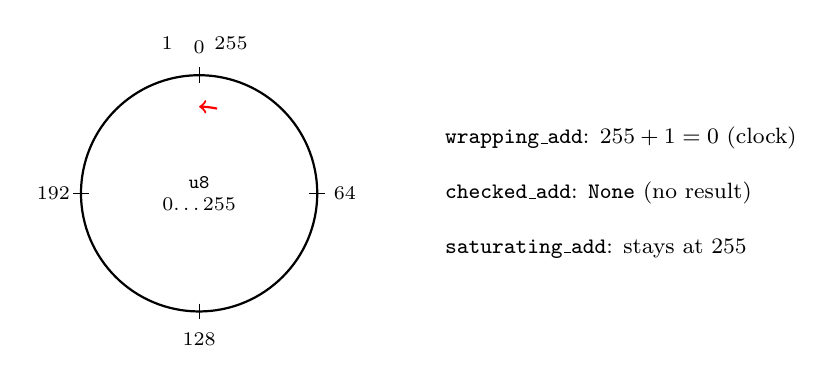
\begin{tikzpicture}[scale=1.0]
 \draw[thick] (0,0) circle (1.5);
 \foreach \a/\t in {90/0,0/64,-90/128,180/192} {
   \node[font=\scriptsize] at (\a:1.85) {\t};
   \draw (\a:1.4)--(\a:1.6);}
 \node[font=\scriptsize] at (102:1.95) {1};
 \node[font=\scriptsize] at (78:1.95) {255};
 \draw[->,thick,red] (78:1.1) arc (78:90:1.1);
 \node[font=\scriptsize,align=center] at (0,0) {\texttt{u8}\\ 0\dots255};
 \node[font=\footnotesize,align=left,anchor=west] at (3,0.7) {\texttt{wrapping\_add}: $255+1=0$ (clock)};
 \node[font=\footnotesize,align=left,anchor=west] at (3,0) {\texttt{checked\_add}: \texttt{None} (no result)};
 \node[font=\footnotesize,align=left,anchor=west] at (3,-0.7) {\texttt{saturating\_add}: stays at $255$};
\end{tikzpicture}
\captionof{figure}{A \texttt{u8} behaves like a clock with $256$ positions. Rust lets you choose what happens at the end.}
\end{center}
With plain \verb!+!, an overflow is a \textbf{panic} (the program stops with an error message) in a debug build and silently wraps in a release build, which is why you decide explicitly whenever the numbers can reach the limits. A classical robot bug: a \verb!u8! counter or an angle in an unsigned type, minus one, at the wrong moment. Floating-point numbers follow the same standard as in Python: \verb!NaN! is not equal even to itself, and \verb!0.1 + 0.2 != 0.3! (Chapter~\ref{ch:py2}).

\section*{Printing}
\verb|println!| replaces \verb!print! and f-strings: names in braces are inserted, and after a colon you write the format.
\begin{center}
\renewcommand{\arraystretch}{1.2}
\begin{tabular}{lll}
\textbf{Rust} & \textbf{Python} & \textbf{result for 3.14159}\\ \hline
\verb!{x}! & \verb!{x}! & \texttt{3.14159}\\
\verb!{x:.2}! & \verb!{x:.2f}! & \texttt{3.14}\\
\verb!{x:8.3}! & \verb!{x:8.3f}! & \texttt{\ \ \ 3.142}\\
\verb!{x:e}! & \verb!{x:e}! & \texttt{3.14159e0}\\
\verb!{n:05}! & \verb!{n:05}! & \texttt{00042} (for 42)\\
\verb!{n:#x}! / \verb!{n:08b}! & \verb!{n:#x}! / \verb!{n:08b}! & \texttt{0x2a} / \texttt{00101010}\\
\verb!{v:?}! & \verb|{v!r}| & debug output of any value\\
\end{tabular}
\end{center}
\verb!{:?}! (and the multi-line \verb!{:#?}!) prints almost any value for debugging, \verb|dbg!(x)| prints the file, the line and the value to the error output.

\section*{Functions}
%rs:funcs
\begin{verbatim}
use std::f64::consts::PI;

fn deg_to_rad(deg: f64) -> f64 {
    deg * PI / 180.0          // no semicolon: this is the return value
}

fn clamp(x: f64, lo: f64, hi: f64) -> f64 {
    if x < lo { lo } else if x > hi { hi } else { x }
}

fn main() {
    let a = deg_to_rad(90.0);
    println!("{a:.4}");
    println!("{}", clamp(1.7, -1.0, 1.0));
    println!("{}", clamp(-3.0, -1.0, 1.0));
}
\end{verbatim}
prints \verb!1.5708!, \verb!1! and \verb!-1!. Parameter types and the return type (after \verb!->!) are always written; inside the function the compiler infers the rest. The last \emph{expression} without a semicolon is the value of the function; \verb!return! is only used for an early exit. In Rust, almost everything is an expression: \verb!if ... else ...! \emph{has a value}, as the conditional expression \verb!a if c else b! of Python has. Both branches must have the same type. A function without \verb!->! returns the empty value \verb!()! (``unit'').

\section*{Control flow}
%rs:loops
\begin{verbatim}
fn main() {
    for i in 0..3 { print!("{i} "); }              // 0 1 2
    println!();
    for i in (0..10).step_by(4) { print!("{i} "); } // 0 4 8
    println!();
    let mut n = 27_u32;
    let mut steps = 0;
    while n != 1 {
        n = if n % 2 == 0 { n / 2 } else { 3 * n + 1 };
        steps += 1;
    }
    println!("steps: {steps}");
    let mut t = 0.0;
    let found = loop {                  // loop: until break
        t += 0.1;
        if t * t > 2.0 { break t; }     // break can return a value
    };
    println!("{found:.1}");
    let joints = ["hip", "knee", "ankle"];
    for (i, j) in joints.iter().enumerate() {
        println!("{i}: {j}");
    }
}
\end{verbatim}
\verb!0..3! is the range $0,1,2$ (the end is excluded, as \verb!range(3)! in Python), \verb!0..=3! includes the end. \verb!for! goes through anything that can be iterated, \verb!.iter()! borrows the elements of an array (Chapter~\ref{ch:rust3}), \verb!.enumerate()! gives index and element. There are no parentheses around the condition, but braces are required. Conditions must be \verb!bool!: \verb!if n {...}! with an integer is an error, you write \verb!n != 0!.

\section*{Collections: tuples, arrays and vectors}
\begin{center}
\renewcommand{\arraystretch}{1.2}
\begin{tabular}{lll}
\textbf{Rust} & \textbf{Python} & \textbf{properties}\\ \hline
\verb!(1, 2.5, 'a')! & \verb!(1, 2.5, 'a')! & tuple, types may differ, fixed length\\
\verb![f64; 3]! & --- & array, fixed length, same type\\
\verb!Vec<f64>! & \verb!list! & growable list, same type\\
\verb!&[f64]! & --- & a view on an array or a vector (``slice'')\\
\end{tabular}
\end{center}
%rsmain:vecs
\begin{verbatim}
    let p = (1.0, 2.5);
    let (x, y) = p;                    // unpacking, as in Python
    let q = [0.0_f64; 4];              // four zeros
    let mut v = vec![3.0, 1.0, 2.0];   // a Vec
    v.push(5.0);
    v.sort_by(|a, b| a.partial_cmp(b).unwrap());
    println!("{x} {y} {q:?} {v:?} len={}", v.len());
    println!("{} {}", v[0], v[v.len() - 1]);
    let total: f64 = v.iter().sum();
    println!("{}", total / v.len() as f64);
\end{verbatim}
prints the numbers \verb!1 2.5 [0.0, 0.0, 0.0, 0.0] [1.0, 2.0, 3.0, 5.0] len=4!, then \verb!1 5! and \verb!2.75!. Indexing outside a vector (\verb!v[10]!) stops the program with a panic and a clear message; it never reads wrong memory. Floats cannot be sorted with \verb!sort()! because \verb!NaN! has no order; \verb!sort_by! with \verb!partial_cmp! says how to compare (the \verb!|a, b| ...! is a small anonymous function, a \emph{closure}, like a Python \verb!lambda!, Chapter~\ref{ch:rust5}).

\section*{A complete example: simulating a spring}
A leg that is pulled back and released behaves like a damped spring, $\ddot x=-k\,x-c\,\dot x$ with $k=4$ and $c=0.1$. We integrate with the simple Euler step (better methods follow in Part~\ref{part:control}): $v\leftarrow v+a\,\Delta t$, $x\leftarrow x+v\,\Delta t$.
%rs:spring
\begin{verbatim}
use std::time::Instant;

fn main() {
    let n: u64 = 50_000_000;
    let dt = 1e-6;
    let (mut x, mut v) = (1.0_f64, 0.0_f64);
    let t0 = Instant::now();
    for _ in 0..n {
        let a = -4.0 * x - 0.1 * v;
        v += a * dt;
        x += v * dt;
    }
    let ms = t0.elapsed().as_secs_f64() * 1000.0;
    println!("x = {x:.6}, v = {v:.6}");
    eprintln!("time = {ms:.0} ms");     // eprintln: standard error
}
\end{verbatim}
After $50$ s of simulated time ($5\cdot10^7$ steps of $1\,\mu$s) the output is \verb!x = 0.068356, v = 0.087540!. Built with \verb!--release! it needs $445$\,ms on our computer (Chapter~\ref{ch:rust1}). The underscore in \verb!50_000_000! only helps reading, and \verb!_! as a loop variable says that we do not need the counter.

\section*{A function on a list of numbers}
Mean and standard deviation of sensor readings. The parameter \verb!&[f64]! means ``a view of some numbers that I only read'' (the \verb!&! is explained in the next chapter). The call passes \verb!&data!.
%rs:stats
\begin{verbatim}
fn mean(xs: &[f64]) -> f64 {
    xs.iter().sum::<f64>() / xs.len() as f64
}

fn std_dev(xs: &[f64]) -> f64 {
    let m = mean(xs);
    let var = xs.iter().map(|x| (x - m).powi(2)).sum::<f64>()
        / (xs.len() - 1) as f64;
    var.sqrt()
}

fn main() {
    let data = vec![9.8, 10.1, 10.0, 9.9, 10.2];
    println!("mean = {:.3}", mean(&data));
    println!("std  = {:.4}", std_dev(&data));
}
\end{verbatim}
prints \verb!mean = 10.000! and \verb!std  = 0.1581!. The sample variance divides by $n-1$ (as \verb!statistics.stdev! in Python). If \verb!xs! is empty, \verb!xs.len() - 1! on an unsigned number would underflow (a panic in debug builds): thinking about the borders of integer types is part of Rust programming.

\begin{aibox}[From Python to Rust: a short dictionary]
\verb!let! is an assignment (immutable), \verb!let mut! a variable you may change; braces instead of indentation; \verb!fn name(a: T) -> R!; \verb!for x in 0..n!; \verb!Vec<T>! is a \verb!list!; \verb|println!("{x}")| is a \verb!print(f"{x}")!; no \verb!None! on every variable (Chapter~\ref{ch:rust4}); no exceptions (Chapter~\ref{ch:rust5}); and a semicolon ends a statement.
\end{aibox}

\section*{Practice problems}
\begin{enumerate}[label=\textbf{\thechapter.\arabic*}]
  \item Create a new project with \verb!cargo new robot_math! and let it print the sum of the numbers $1$ to $100$. Which command compiles without running?
  \item What do these expressions give? \verb!10 / 4!, \verb!10.0 / 4.0!, \verb!10 % 4!, \verb!-10 % 4!, \verb!(-10_i32).rem_euclid(4)!, \verb!2.9_f64 as i32!, \verb!-2.9_f64 as i32!.
  \item What is \verb!250_u8 + 10! in a release build? How would you write it so that the result is $255$ (``stay at the limit'')? How if you want to know that the limit was exceeded?
  \item Why does \verb!let x: f64 = 2; ! not compile? Give two ways to fix it.
  \item Write a function \verb!fn rad_to_deg(rad: f64) -> f64! and a function \verb!fn wrap_angle(deg: f64) -> f64! that maps any angle to the range $[-180,180)$. Test with $190$, $-190$, $540$.
  \item Write a program that prints the first $10$ values of the sequence $x_{n+1}=x_n/2+1$ with $x_0=0$, one per line with three decimals.
  \item Port this Python function to Rust, with types. \verb!def mean_abs(xs): return sum(abs(x) for x in xs) / len(xs)!. What happens in Python and in Rust (the compiler does not forbid it) if the list is empty? Which values would you return?
  \item A \verb!Vec<f64>! contains the distances of seven ultrasonic sensors. Write a function that returns the smallest value, without using a ready-made \verb!min! function. Why is the result for an empty vector a problem? (Chapter~\ref{ch:rust4} gives the answer; think about it now.)
  \item Which of these lines are errors, and why? (a) \verb!let a = 5; a += 1;! (b) \verb!let b: i32 = 5.0;! (c) \verb!let c = 5 + 2.5;! (d) \verb!let d = [1, 2, 3]; let e = d[5];! (e) \verb!if 1 { }!
  \item[\textbf{\thechapter.10}$\star$] Euler integration of a damped spring has an error. Write a program that simulates $T=10$\,s with $\Delta t\in\{0.1,\,0.01,\,0.001\}$ (spring constant $k=4$, damping $c=0.1$, $x_0=1$, $v_0=0$) and prints $x(T)$ for each. The exact solution is $x(t)=e^{-ct/2}\left(\cos\omega t+\frac{c}{2\omega}\sin\omega t\right)$ with $\omega=\sqrt{k-c^2/4}$. Print also the absolute error. By what factor does the error shrink when $\Delta t$ becomes ten times smaller?
\end{enumerate}
